\section{Co-Saliency based Color Design}
Given $N$ ($N\geq 2$) categorical visualizations with the same class labels (or a subset thereof), the $j$th visualization has $M$ classes and $n_j$ data items $\{\mathbf{x}^j_1, \cdots, \mathbf{x}^j_{n_j}\}$, where each $\mathbf{x}^j_t$ has a label
$l(\mathbf{x}^j_t)$ and the $i$-th class (with $n^j_i$ data points) consists of $\{\mathbf{x}_{i,1}^j, \cdots , \mathbf{x}_{i,n^j_i}^j\}, i \in  \{ 1, \cdots, m \} $.
For standard bar and line charts, $M$ is equal to $n_j$ but it is often smaller than $n_j$ for scatterplots.
All visualizations use the same  background color $\mathbf{c}_b$ and the same color mapping scheme $\tau: L \mapsto c$. Our goal is to find the best mapping $\tau$ that supports an effective comparison of multiple categorical visualizations.
% scatterplots.

In line with the design requirements for natural image comparison and categorical data visualization~\cite{Jacobs10,Gleicher18,Lu21},
%~\cite{itti1998model,cheng2014global,zhang2018review},
our problem is formulated based on the following three design requirements:
\begin{enumerate}[label=(\roman*),nosep]
\item \textbf{DR1:} highlighting the most concerned classes between visualizations as much as possible for an efficient comparison;
\item \textbf{DR2:} maximizing the visual discrimination between classes in the individual visualizations for an efficient exploration of multi-class data; and
\item \textbf{DR3:} providing flexible interactions for the exploration of relationships among the compared datasets.
%co-salient classes should follow the principles of visual salience in individual visualizations so that the co-salient classes can be easily identified.
\end{enumerate}
Although visual comparison is an essential part of interactive data analysis, most of  the existing  colorization techniques~\cite{Gramazio17, Lu21} attempt to meet DR2. The key challenge in meeting DR1 is that we need a proper model to characterize the most salient features in multiple visualizations.
To address this issue, we propose our %a categorical visualization
co-saliency model that calculates the saliency of each data item in the context of other similar visualizations. Integrating this model into the objective of a state-of-the-art color mapping generation framework~\cite{Lu21}, we can
generate proper color mappings that highlight salient differences between juxtaposed categorical visualizations while fostering a better visual discrimination of classes.

\subsection{Co-saliency for Multi-class Scatterplots }
Following the definition of image co-saliency~\cite{Jacobs10}, we model class co-saliency with two factors: class importance between visualizations and class contrast within visualizations. The class importance describes how much each class should stand out from the visualization.
Class contrast describes how much each class stands out from neighboring classes and the background,
which is similar to perceptual class separability~\cite{Aupetit02,Wang2018}. Hence,
we define two types of class contrasts: a local contrast with neighboring classes and a contrast with the background.

Since point-based representations are very general in 2D visualization, we use two ($N=2$) horizontally juxtaposed scatterplots to illustrate our method.
Analogous to bottom-up image co-saliency models~\cite{Jacobs10,Fu13}, the co-saliency of the $i$th class is defined as the product between the class importance and  class contrast scores to emphasize the target class and the co-saliency for $M$ classes:
\begin{equation}
% E_{CoS} = \sum_i   \sum_j (1-\lambda) \alpha^j_i  \exp(\theta_i) + \lambda \beta_i  f(\theta_i)
E_{CoS} = \sum_i^M    \left(\sum_j^N \frac{1}{n^j_i}\bigg(\lambda \alpha^j_i\exp(\theta_i) + (1-\lambda) \beta^j_i f(\theta_i) \bigg) \right),
	\label{eq:cosaliency}
\end{equation}
where $\theta_i$ is the importance of the $i$th class,
$n^j_i$ is the number of points of the $i$th class in the $j$th scatterplot,
$\alpha^j_i$ is the local contrast with the neighboring classes of the $i$th class in the $j$th scatterplot, $\beta^j_i$  is the contrast of the class to the background, and $\lambda$ is the weight between them. The weight $1/{n^j_i}$  is used to alleviate class imbalances  so that  classes with small numbers of points and large changes can be highlighted.

To better support DR1, we apply an exponential function to enlarge the weight of structural class changes, while using a piecewise function weighting the background contrast:
\begin{align}
f(\theta_i) =  \left\{ \begin{array}{ll}
\exp(\theta_i) & \textrm{if $\theta_i>\kappa$}\\
-\exp(\theta_i) & \textrm{else}
\end{array} \right.
\label{eq:energyfunc}
\end{align}
where $\kappa$ is a user-specified threshold with a default of zero. The reason for the two different weighting schemes is that classes with less or no changes might be treated as the background by viewers~\cite{zhang2018review}. To suppress the saliency of such classes, we introduce a negative importance for them.

\vspace{2mm}
\noindent\textbf{Local Contrast}.
%Given the $j$th scatterplot, we define the local class contrast based on the point distinctness~\cite{Lu21}.
%Here, we briefly describe its computation process and
%refer to Lu et al.~\cite{Lu21} for more details.
%Given the data point $\mathbf{x}^j_t$, its distinctness is defined as the sum of the color differences from its neighbourhoods weighted by the inverse Euclidean distance.
%Then, the distinctness of the $i$th class is the sum of all points with the same class label in the scatterplot, which is further normalized by ${n^j_i}$.
Given the $j$th scatterplot, we define the local class contrast based on the $\alpha$-shape based point distinctness~\cite{Lu21}.  For each data point $\mathbf{x}^j_t$, we define its point distinctness  as:
\begin{align}
 \gamma (\mathbf{x}^j_t)=\frac{1}{|\Omega^j_t|} \sum_{\mathbf{x}^j_p \in \Omega^j_t}  \frac{\Delta\epsilon(\tau(l(\mathbf{x}^j_t)),\tau(l(\mathbf{x}^j_p)))}{d(\mathbf{x}^j_t,\mathbf{x}^j_p)} \nonumber ,
\end{align}
where $\Omega^j_t$ is set of $k$ nearest neighbors of $\mathbf{x}^j_t$, $\tau(l(\mathbf{x}^j_p))$ is the color of $\mathbf{x}^j_p$,  $d$ is the Euclidean distance and $\Delta\epsilon$ is the CIELAB color distance~\cite{sharma2005ciede2000}.
For the $i$th class, its local contrast is the sum of all points with the same class label in the scatterplot:
\begin{align}\label{eq:nc}
 \phi^j_i = \frac{1}{n_i^j}\sum^{n_j}_{t}\gamma(\mathbf{x}^j_t) \delta(l(\mathbf{x}^j_t),i),
\end{align}
where $\delta(l(\mathbf{x}^j_t),i)$ is one if the class label $l(\mathbf{x}^j_t)$ is $i$ and else zero.

If a class overlaps with different classes, the local contrast value will be high and the value will be small for a well separated class. Hence, the black class  in the  two scatterplots shown in Fig.~\ref{fig:map}(a)  has a low contrast value (see Fig.~\ref{fig:map}(b)) and the cyan class has a large value.


%\begin{align}\label{eq:pdc}
% \alpha^j_i = \frac{1}{n^j_i}\sum^{n_j}_{p}\gamma(\mathbf{x}^j_p) \delta(l(\mathbf{x}^j_p),i)
%\end{align}
%where $\delta(l(\mathbf{x}^j_p),i)$ is one if the class label $l(\mathbf{x}^j_p)$ is $i$ and else zero.
%
%
%However, KNNG cannot reflect the contrast among classes without any overlap. For example,  in Fig.~\ref{fig:knng}(a) the contrast between the blue class and the brown classes cannot be reflected.
%To address this issue, we introduce an additional class-center based contrast cue~\cite{Fu13}.
%Suppose the center of the $i$th class in this scatterplot is $\mu^j_i$, the class contrast is:
%\begin{align}\label{eq:cc}
% \varphi^j_i =  \frac{1}{M}\sum^M_{m}\frac{\Delta\epsilon(\tau(i),\tau(m))}{||\mu^j_m -\mu^j_i ||},
%\end{align}
%which assigns large weights to nearby classes and small ones to far-away classes. The final class contrast of the $i$th class is:
%\begin{align}\label{eq:pd}
% \alpha^j_i  = \phi^j_i  + \omega \varphi^j_i,
%\end{align}
%where the weight $\omega$ is 1.0 in our experiment.

\vspace{2mm}
\noindent\textbf{Background Contrast}.
The contrast to the background is based on the so-called point non-separability $\rho (\mathbf{x}^j_t)$ (rf.~\cite{Wang2018}), which is defined as the difference between two  separation degrees:
\begin{align}
\rho(\mathbf{x}^j_t)&= b(\mathbf{x}^j_t)-a(\mathbf{x}^j_t) \ ,
\end{align}
where $b(\mathbf{x}^j_t)$ is the between-class separation degree and $a(\mathbf{x}^j_t)$ is the within-class separation degree.
% of $\mathbf{x}^j_t$.
The measures are defined as weighted sums of  color differences of $\mathbf{x}^j_t$ with its neighborhood from the same and different classes:
\begin{align}
a(\mathbf{x}^j_t)&=\frac{1}{|\Omega^j_t|}\sum_{\mathbf{x}^j_p \in \Omega^j_t } \frac{\delta(l(\mathbf{x}^j_t), l(\mathbf{x}^j_p))
\Delta\epsilon(\tau(l(\mathbf{x}^j_t)),\mathbf{c}_b)
}{d(\mathbf{x}^j_t,\mathbf{x}^j_p)} , \;\;
b(\mathbf{x}^j_t)=\frac{1}{|\Omega^j_t|}\sum_{\mathbf{x}^j_p \in \Omega^j_t } \frac{(1-\delta(l(\mathbf{x}^j_t), l(\mathbf{x}^j_p)))\Delta\epsilon(\tau(l(\mathbf{x}^j_t)),\mathbf{c}_b)}{d(\mathbf{x}^j_t,\mathbf{x}^j_p)}  .\nonumber
\end{align}

When most neighbor points of $\mathbf{x}^j_t$ have the same label as $\mathbf{x}^j_t$,  $\rho (\mathbf{x}^j_t)$ is negative.
% and vice versa.
%the corresponding class has large within-class separability and small between-class separability and thus $\rho (\mathbf{x}^j_t)$ is negative; and vice versa.
However, such a negative $\rho (\mathbf{x}^j_t)$ makes the optimization in Eq.~\ref{eq:cosaliency} meaningless, and the corresponding classes might be highlighted no matter how large the change of this class is.
To address this issue, we use an exponential function to let $\rho (\mathbf{x}^j_t)$  always be positive while maintaining the monotonicity of the function. Accordingly, we define
%\begin{align}\label{eq:ctb}
% \rho (\mathbf{x}^j_t)=\frac{1}{|\Omega^j_t|} \sum_{\mathbf{x}^j_p \in \Omega^j_t}  \frac{(1-2\delta(l(\mathbf{x}^j_t),l(\mathbf{x}^j_p)))\Delta\epsilon(\tau(l(\mathbf{x}^j_t)),\mathbf{c}_b)}{d(\mathbf{x}^j_t,\mathbf{x}^j_p)} ,
%\end{align}
the contrast to the background of the $i$th class as:
\begin{align}\label{eq:ctbc}
 \beta^j_i = \frac{1}{n^j_i}\sum^{n_j}_{t} \exp(\rho(\mathbf{x}^j_t)) \delta(l(\mathbf{x}^j_t),i).
\end{align}
%where
%$\delta(l(\mathbf{x}^j_p),i)$ is one if the class label $l(\mathbf{x}^j_p)$ is $i$ and else zero.
%In doing so, all classes have positive background contrast value.
As illustrated in Fig.~\ref{fig:map}(c), well-separated classes with large color differences from the background have large background contrast (blue and black classes), whereas the pink and cyan classes have relatively large background contrast values with a medium class separation.


%\begin{wrapfigure}{r}{0.28\columnwidth}
%	\vspace{-5mm}
%	\centering
%	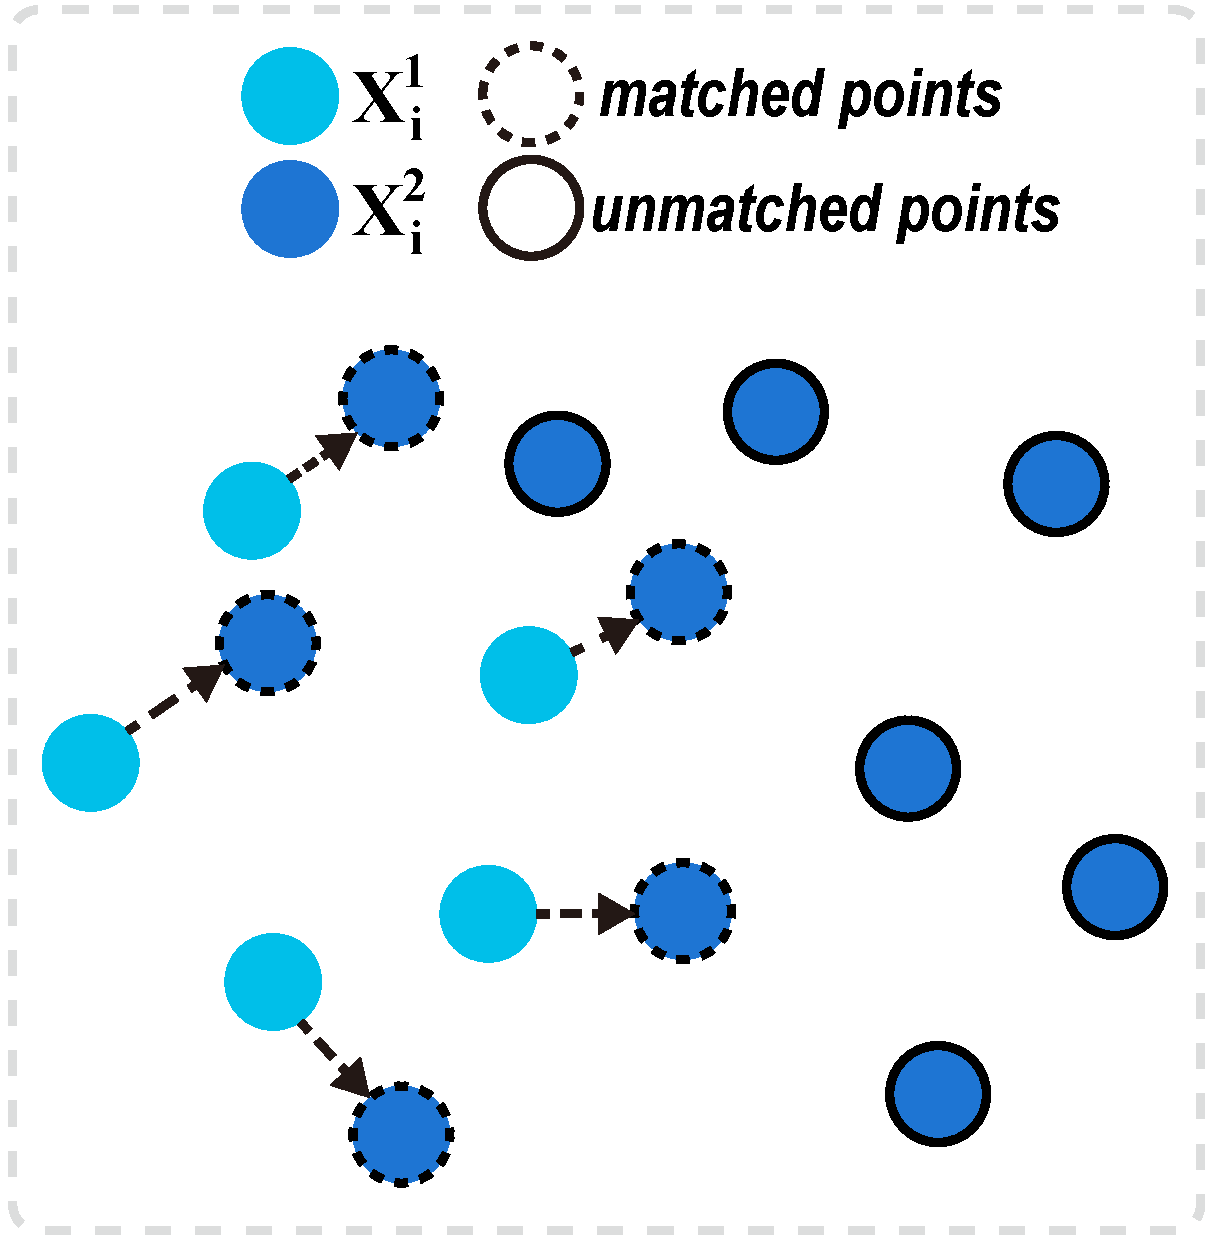
\includegraphics[width=0.28\columnwidth]{class-change-degree}
%	\vspace*{-8mm}
%	\caption{An one-to-one mapping for computing the changes between two classes.}
%	\vspace*{-2mm}
%	\label{fig:class-change-degree}
%\end{wrapfigure}
 %Since $\rho (\mathbf{x}^j_t)$ might be a negative value which will be influenced by Eq.~\ref{eq:piecewiseFunc}, we apply an exponential function to transfer it to positive while maintains the monotonicity.

\vspace{1.5mm}
\noindent\textbf{Class Importance}.
Class importance reflects whether a class should be highlighted or not. It can be specified by user or by some measures. In our paper, as a default we use the class change degree to represent the importance of each class.
To quantify how users perceive structural changes of classes, we measure the difference between the class distributions in two scatterplots using the Earth Mover's Distance (EMD)~\cite{rubner2000earth}, a perceptual metric.
Suppose the $i$th  class with two representations by two sets of points $\mathbf{X}^1_i = \{\mathbf{x}_{i,1}^1, \cdots , \mathbf{x}_{i,n^1_i}^1\}$ and $\mathbf{X}^2_i = \{\mathbf{x}_{i,1}^2, \cdots , \mathbf{x}_{i,n^2_i}^2\}$.
Taking the Euclidian distance between points as the cost, we need to  minimize the total matching cost
\begin{align}
 H(\mathbf{X}^1_i, \mathbf{X}^2_i)  = \min_\chi \sum_t d(\mathbf{x}_{i,t}^1, \mathbf{x}_{i,\chi(t)}^2), \nonumber
\end{align}
which constrains one-to-one mappings $\chi$ between points %(see an illustration in Fig.~\ref{fig:class-change-degree}).
This is the classic bipartite matching problem, which can be solved by the Hungarian method~\cite{kuhn1955hungarian}.
When the number of points of two sets is not equal, we further take the difference between the number of points into account. In doing so, the class change degree contains  positional changes and changes of element numbers:
\begin{align}\label{eq:cm}
 \theta_i= \frac{H(\mathbf{X}^1_i, \mathbf{X}^2_i) }{\min\{n^1_i, n^2_i\}} + \nu \frac{||n^1_i- n^2_i||}{\max\{n^1_i, n^2_i\}},
\end{align}
where both terms range within [0,1] and $\nu$ is 1.0 as the default value.


\begin{figure*}[!tb]
\centering
\includegraphics[width=\linewidth]{figures/saliencymap}
\caption{Main components for computing co-saliency maps: For the two input scatterplots (a), our class-based co-saliency (e) is generated by fusing  local contrast (b),  background contrast (c),  and class change degree (d). Brightness of points denotes value.
	% and vice versa.
}
\vspace*{-3mm}
\label{fig:map}
\end{figure*}
\vspace{1.5mm}

Fig.~\ref{fig:map} shows an example of two 8-class scatterplots with three  changing classes (orange, blue and black). Combining the class change degree with the two above-given contrast measures allows us to highlight salient differences and maintain the visual discrimination of the classes (see Fig.~\ref{fig:map} (e)).
